% Chapter 8

\chapter{Experiment} % Write in your own chapter title
\label{Chapter8}
\lhead{Chapter 8. \emph{Experiment}}

The experiment has the identical hardware and software environment as described in the weather classification project.

\section{Dataset}

We generate $1000$ raw RGB images with size $16 \times 16$. $40$ images are reserved for testing and $960$ images are used for training. Each image has $3$ labels $y_i \in (-1, 1)$ representing three attributes, red, green and blue. If the image has a colour attribute, the corresponding label value is $1$, otherwise $-1$.

\section{Details of Network}

The neural network is built from scratch up. First, we need to determine how many layers needed for the network. In \cite{lippmann1987introduction}, Lippmann has proved that two hidden layers are able to create classification regions of arbitrary desired shape. However, Kolmogorov \citep{kolmogorov1963representation} showed that the superposition of continuous one-dimension function can represent a continuous function with several variables. Then we set up a neural network with one fully connected hidden layer between the input and output layers.
\begin{figure}[!htb]
\centering
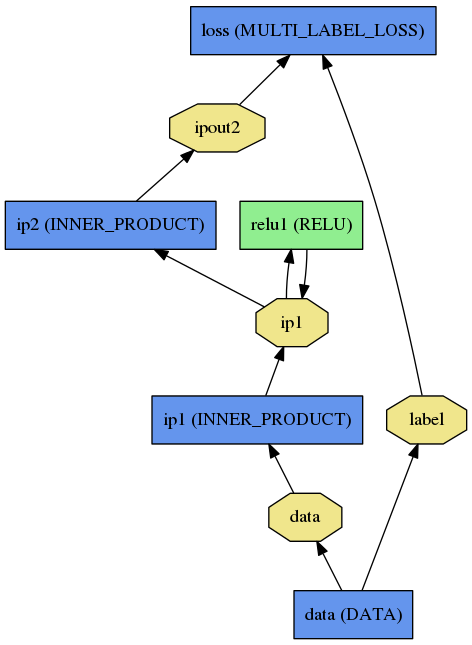
\includegraphics[width=0.8\textwidth]{multilabel-topology.png}
\caption{\label{fig:MLtopology}Network Topology}
\end{figure}
Between two layers, we put a ReLU layer to apply the non-saturating activation function $f(x) = max(0,x)$ which helps the decision function increase the non-linear properties.

Following that, it needs to determine how many neurons needed in the hidden layer. The number of neurons in the hidden layer depends mainly on
\begin{enumerate}
  \item Number of input and output neurons
  \item Number of training samples
  \item Layer connecting types
  \item Training algorithms
  \item Type of activation function
  \item Regularisation
\end{enumerate}
It is difficult to determine the best number of hidden neurons without evaluating several trained models and comparing the generalisation error rates among the models. Lacking hidden neurons will lead a high training error rate and poor generalisation performance because of underfitting and high bias. On the other hand, exceeding neurons will achieve a high training error rate and poor generalisation performance because of overfitting and high variance. One of crucial considerations is to evaluate the hidden neuron effects on the bias/variance trade-off.

There are many rules of thumb to determine the number of hidden neurons \citep{heaton2008introduction}
\begin{enumerate}
  \item $\frac{2}{3}$ of the sum of the input neurons plus the output neurons.
  \item Less than twice the size of the input layer.
  \item Following geometric pyramid rule, between the number of input neurons and the output neurons.
\end{enumerate}
It is time consuming to find the optimal number of hidden neurons. We will start from a number of neurons which is small and increase the number gradually by evaluating the performance of network.

The different layers are fully connected because we want to map each patch to the labels of the image. The information of each colour distributes in different positions of the image. The values of the weights and bias are initialised randomly. For weights, the $xavier$ algorithm is applied to determine the scale of initialisation depending on the number of input and output neurons. The bias is simply initialised as a constant $0$. The batch size is $40$.

In the training process, the base learning rate is $0.0001$. The learning rate of weights is equal to base learning rate, while the learning rate of bias is two times of the base learning rate. The parameter momentum is $0.9$ to smooth the weight updating curve across iterations so that the learning process will be fast. The weight decay is $0.0005$.

The evaluation metric is label-metric. Each label will be counted separately and statistics will be calculated in total.

\section{Results}

The test results with different number of hidden neurons are showed in table \ref{tb:tMLtestneurons} and Figure \ref{fig:MLtestneurons}. Results show that the model with 200 neurons in the hidden layer has the best performance.
\begin{table}
\centering
\begin{tabular}{l*{6}{c}}
Neuron number              & Sensitivity & Specificity & Harmonic Mean & Precission & F1 Score  \\
\hline
4 				& 0.9245 & 0.9552 & 0.9396 & 0.9423 & 0.9333   \\
50              & 0.9245 & 0.9701 & 0.9468 & 0.9608 & 0.9423   \\
100             & 0.9623 & 0.9701 & 0.9662 & 0.9623 &  0.9623  \\
150             & 0.9057 & 0.9552 & 0.9298 & 0.9412 &  0.9231   \\
200             & 0.9811 & 1.0000 & 0.9905 & 1.0000 &  0.9905   \\
250             & 0.9434 & 1.0000 & 0.9709 & 1.0000 &  0.9709   \\
300             & 0.9811 & 0.9701 & 0.9756 & 0.9630 &  0.9720   \\
350             & 0.9434 & 0.9701 & 0.9566 & 0.9615 &  0.9524   \\
400             & 0.8868 & 0.9701 & 0.9266 & 0.9592 &  0.9216   \\
450             & 0.9245 & 0.9701 & 0.9468 & 0.9608 &  0.9423   \\
500             & 0.9622 & 0.9701 & 0.9662 & 0.9623 &  0.9623   \\
\end{tabular}
\caption{\label{tb:tMLtestneurons}Test results for different number of hidden neurons.}
\end{table}
\begin{figure}[htb]
\centering
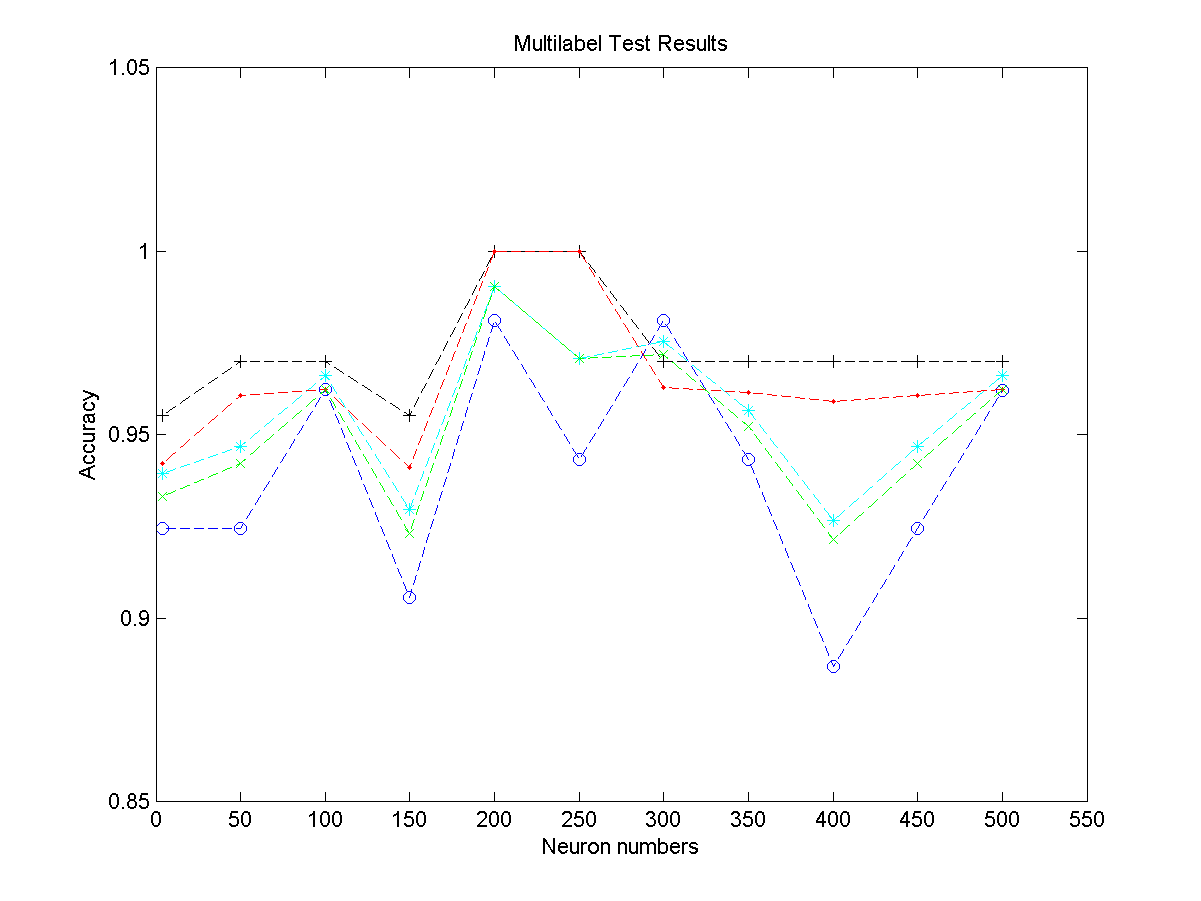
\includegraphics[width=0.8\textwidth]{MLtestneurons}
\caption{\label{fig:MLtestneurons}The test results for different number of hidden neurons. Blue circle for Sensitivity. Black plus for Specificity. Cyan star for Harmonic Mean. Red dot for Precission. Green x for F1 Score.}
\end{figure}


\begin{figure}[htb]
\centering
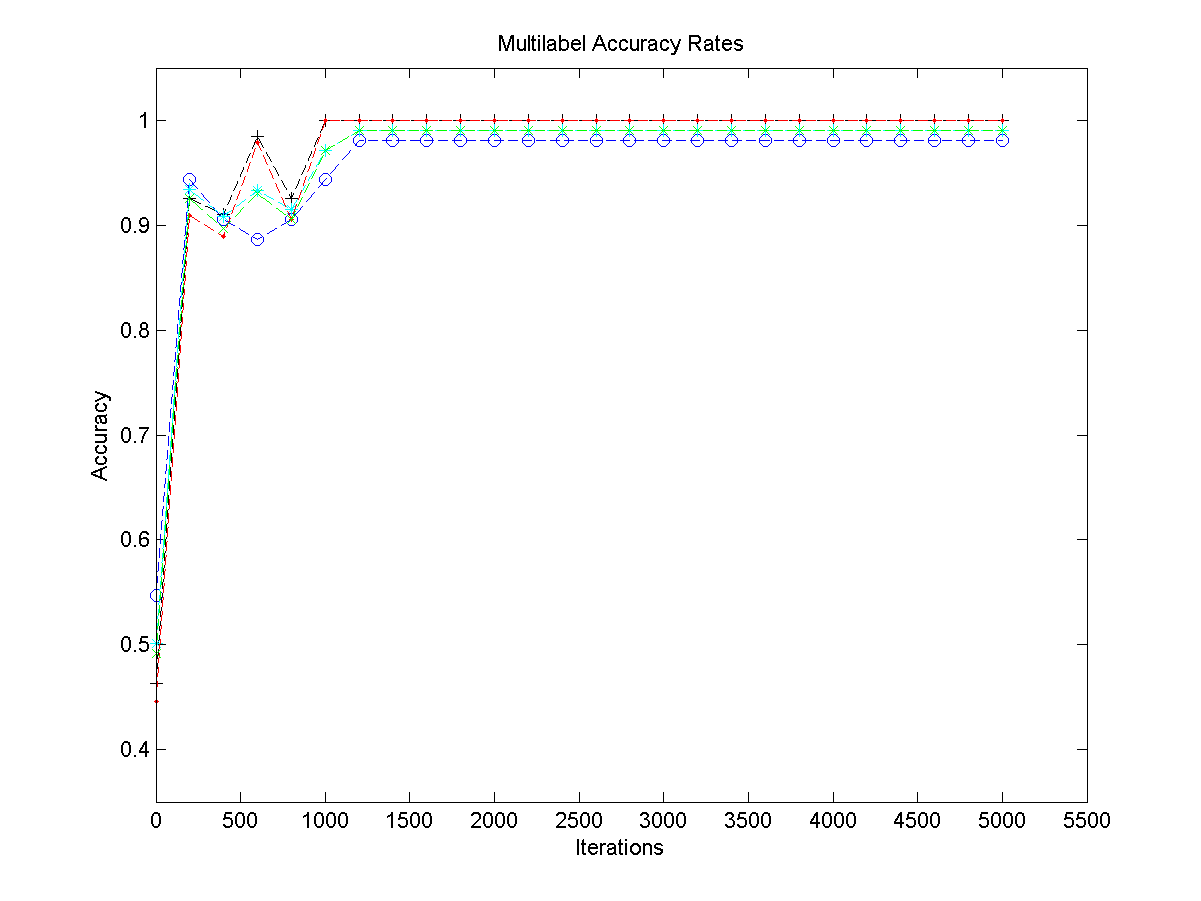
\includegraphics[width=0.8\textwidth]{MLLearningRates}
\caption{\label{fig:MLLearningRates}The learning speed for 200 neurons in the hidden layer. Blue circle for Sensitivity. Black plus for Specificity. Cyan star for Harmonic Mean. Red dot for Precission. Green x for F1 Score.}
\end{figure}
In Figure \ref{fig:MLLearningRates}, it shows that the learning speed is quick. After reaching high accuracy, the accuracy reverses stable. 

In figures \ref{fig:MLROCCurve} \ref{fig:MLROCCurveExt}, the ROC curve of test results shows that the average accuracy is high. In detail, the micro-accuracy for label $0$(red) is the highest, followed by accuracies for label $1$(green) and label $2$(blue). 
\begin{figure}[htb]
\centering
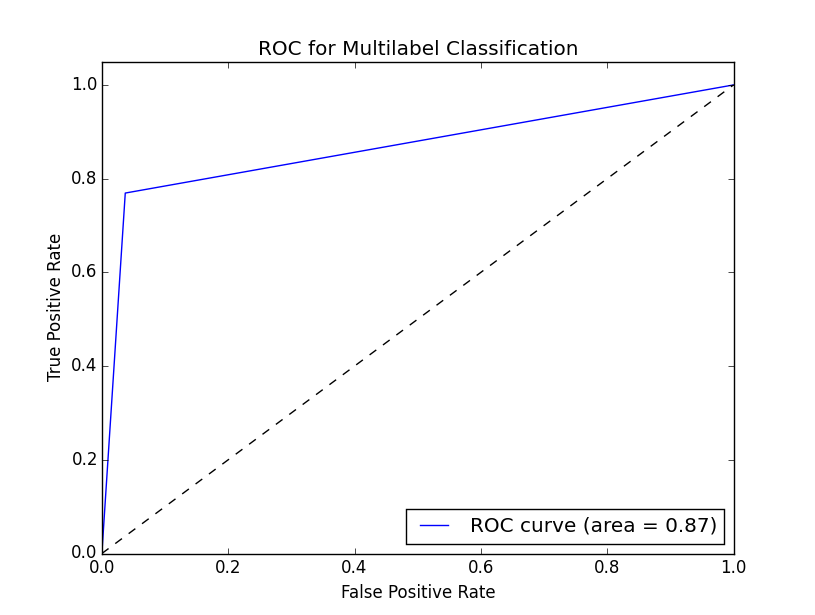
\includegraphics[width=0.8\textwidth]{ROCMultilabel}
\caption{\label{fig:MLROCCurve}The ROC curve for 200 hidden neurons}
\end{figure}

\begin{figure}[htb]
\centering
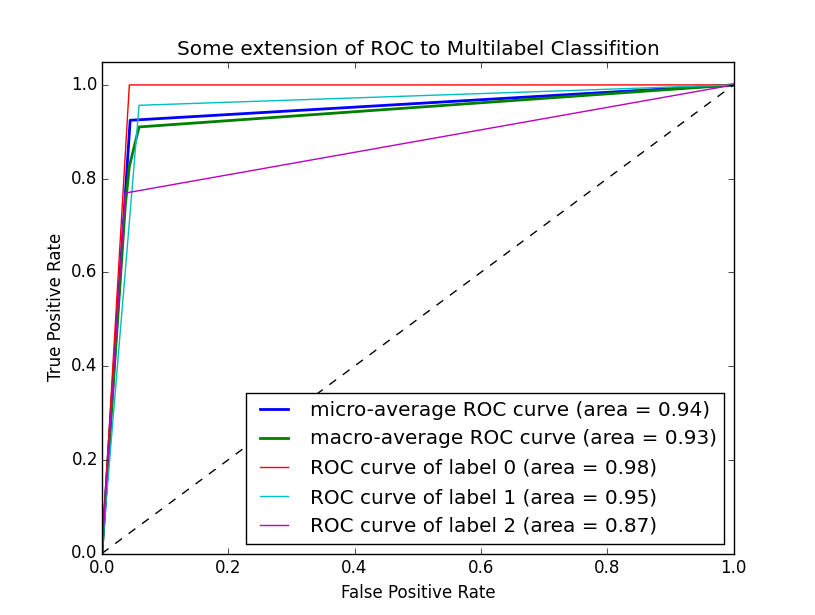
\includegraphics[width=0.8\textwidth]{ROCMultilabelExt}
\caption{\label{fig:MLROCCurveExt}The ROC curve for 200 hidden neurons}
\end{figure}

\section{Conclusion and Future Work}

We have presented an effective approach to classifying multi-label images. With increasing label numbers, the correlation between data and labels is complex. A neural network maps data and labels efficiently and accurately. The updated loss function evaluates the model efficiently and quickly leads to optimisation.

The experiment shows that the neural network is able to do complex multi-label classification perfectly. In the experiment, classifying the artificial images achieves the high generalisation performance. It needs to update the network architecture for practical datasets in the future.












